\documentclass[a4paper]{article}

\usepackage{fullpage}
\usepackage{parskip}
\usepackage{tikz}
\usepackage[utf8]{inputenc}
\usepackage[spanish]{babel}
\usepackage{amsmath}
\usepackage{hyperref}

\title{Ecuación de transferencia radiativa}
\author{Francisco Tapia}
\date{\today}

\begin{document}

\maketitle

\section{Introducción}

El mecanismo más importante para transportar energía a traves de la atmósfera estelar es el transporte radiativo, el cual gobierna el campo de radiación in un medio que absorbe, emite y dispersa la radiación.

\section{Intensidad específica} 

La cantidad de energía, dE$_{\nu}$, en un intervalo específico de frecuencia ($\nu,\nu+d\nu$), el cual es transportado a través de un elemento de área dA en dirección a un elemento de ángulo sólido d$\omega$ durante un tiempo dt (figura \ref{fig:1.2}). Esta energía dE$_{\nu}$, es expresada en términos de intensidad específica I$_{\nu}$ como


\begin{equation} \label{eq1}
\begin{split}
    %dP & =I_\nu cos\theta d\Omega d\sigma d\nu
    dE_{\nu} &= I_{\nu} dA d\omega d\nu dt \hat{r} \cdot \hat{n}
\end{split}
\end{equation}

donde $\hat{r} \cdot \hat{n}$ = cos($\theta$) = $\mu$ y $\theta$ es el ángulo entre la dirección considerada y la normal a dA. Tenemos entonces

\begin{equation} \label{eq2}
\begin{split}
   %I_\nu  & = \frac{dP}{cos\theta d\Omega d\sigma d\nu}
   dI_\nu  & = \frac{dE}{dA d\omega d\nu dt cos(\theta)}
\end{split}
\end{equation}


Se espera de la definición de intensidad que en un medio que absorbe, emite y dispersa la radiación I$_{\nu}$ varíe de un punto a otro en función de su dirección y el tiempo. Si tenemos un superficie plana, suponemos una emisión isotrópica , en cuyo caso es conveniente utilizar una simetría esférica (figura \ref{fig:1.2}). Para este caso la intensidad (I$_{\nu}$) se puede escribir como

\begin{equation} \label{eq2.1}
\begin{split}
   I_\nu  & = I_\nu(\theta,\phi,t) 
\end{split}
\end{equation}


\begin{figure}[h]
\centering
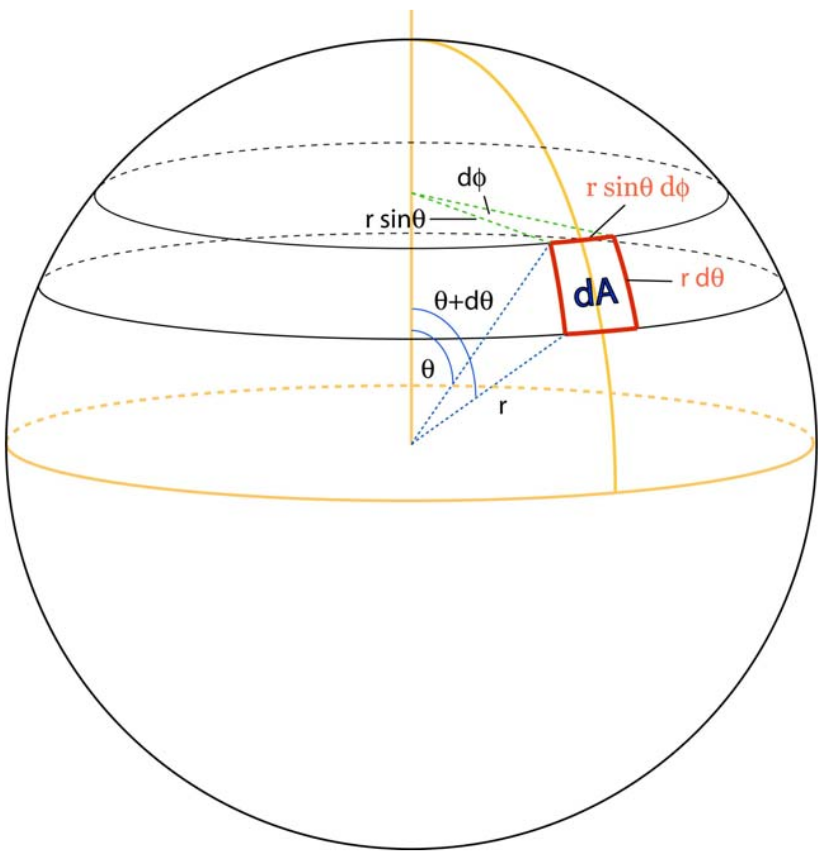
\includegraphics[width=8cm]{emisionesferica.png}
\caption{Definición de brillo}
\label{fig:1.2}
\end{figure}

Si integramos la ecuación \ref{eq1} ($dE_\nu \sim I_\nu cos \theta d\omega$), obtenemos el flujo total de energía sobre el ángulo sólido $\Omega_{f} = 4\pi$ subtendido por la fuente

\begin{equation} \label{eq3}
\begin{split}
   %S_\nu  & = \int_{\Omega_{\nu}} I_{\nu}(\theta,\varphi) cos\theta d\Omega
   F_\nu  & = \int_{\Omega} I_{\nu}(\theta,\phi,t) cos\theta d\omega = \int_{0}^{2\pi} \int_{0}^{\pi} I_{\nu}(\theta,\phi,t) cos\theta sin\theta d\theta d\phi
\end{split}
\end{equation}


La densidad de flujo es medida en unidades de $erg\;cm^{-2}\;Hz^{-1}\;ster^{-1}$.%$Wm^{-2}Hz^{-1}ster^{-1}$.
Usualmente la densidad de flujo de radio fuentes es muy pequeña. Especialmente en las radio fuentes astronómicas se utiliza el Jansky (Jy) 

\begin{center}
   1 Jy = $10^{-26}Wm^{-2}Hz^{-1}=10^{-23}ergs^{-1}cm^{-2}Hz^{-1}$
\end{center}
 
Consideramos una esfera con un brillo uniforme $I_{\nu}$ con un radio R. La densidad de flujo total recibido por un observador a una distancia r es entonces de acuerdo a \ref{eq3} 

\begin{equation} \label{eq4}
\begin{split}
   F_\nu  & = F^{+} - F^{-}
\end{split}
\end{equation}

De la ecuación \ref{eq4} tenemos un flujo positivo y un negativo (figura \ref{fig:1.3}). El único flujo que llega a el observador es el flujo positivo por lo tanto

$$F^{+} = \pi I_\nu$$

El flujo total que lleva al observador considerando simetría esférica donde R es el radio de la esfera y r es la distancia a la que se encuentra el observador. Después de integrar (\ref{eq4}) obtenemos

\begin{equation} \label{eq5}
   F^{obs}_{\nu} = \pi I_{\nu} sin^{2}\theta_{c} = \left(\frac{ R}{r}\right)^2 \pi I_{\nu} 
\end{equation}

donde

\begin{center}
   $sin\theta_{c}$  = $\frac{R}{r}$
\end{center}

\begin{figure}[h]
\centering
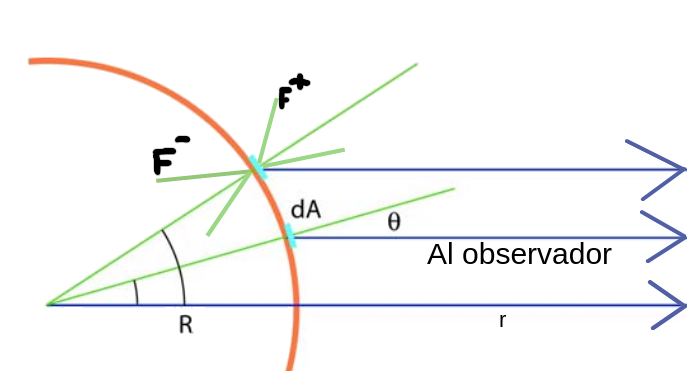
\includegraphics[width=5cm]{fig2.png}
\caption{Simetría esférica}
\label{fig:1.3}
\end{figure}

\newpage   
\section{Ecuación de Transferencia Radiativa}\label{ecu-tra-ra}

Para conocer el cambio de la intensidad a lo largo de la línea de visión, es decir $\mu$=1, se introduce un término de pérdida d$I_{\nu -}$ y un término de ganancia d$I_{\nu +}$ y los definimos como:

\begin{center}
d$I_{\nu -}$ = -$\kappa_{\nu} I_{\nu}$ds\\
d$I_{\nu +}$ = $\varepsilon_{\nu}$ds
\end{center}

por lo cual

\begin{center}
d$I_{\nu}$ = d$I_{\nu -}$ + d$I_{\nu +}$
\end{center}

Si tomamos un elemento de anchura ds y usamos las ecuaciones \ref{eq1} y \ref{eq3} tenemos que

\begin{center}
[$I_{\nu}$(s+ds)-$I_{\nu}$(s)]$d\sigma d\nu d\Omega$ = [$-\kappa_{\nu} I_{\nu} + \varepsilon_{\nu}$]$d\sigma d\nu d\Omega ds$
\end{center}

de la cual resulta la ecuación de transferencia

\begin{equation} \label{eq6}
\boxed{\frac{dI_{\nu}}{ds} = -\kappa_{\nu} I_{\nu} + \varepsilon_{\nu}}
\end{equation}

Si el elemento infinitesimal está en equilibrio térmico local, podemos usar la ley de Kirchhoff

\begin{equation} \label{eq7}
S_{\nu}(T) = \frac{\varepsilon_{\nu}}{\kappa_{\nu}}
\end{equation}

Definimos la profundidad óptica como

\begin{equation} \label{eq8}
\tau_{\nu} := \int_{0} ^{s} -\kappa_{\nu} ds
\end{equation}

%Usando \ref{eq8} podemos escribir la ecuación de transferencia radiativa como

%\begin{equation} \label{eq9}
%\boxed{\frac{dI_{\nu}}{d\tau} = I_{\nu} - S_{\nu}(T)}
%\end{equation}

La solución general de la ecuación de transferencia radiativa se obtiene multiplicando por exp(-$\tau_{\nu}$) e integrando (\ref{eq6})


\begin{equation} \label{eq10}
I_{\nu}(\tau_{2}) = I_{\nu}(\tau_{1}) e^{-(\tau_{1} - \tau{2})} - \int_{\tau_{1}}^{\tau_{2}} S_{\nu}(T) e^{-(\tau_{\nu} - \tau{2})} d\tau_{\nu}
\end{equation}

\begin{equation} \label{eq11}
I_{\nu}(\tau_{2}) = I_{\nu}(\tau_{1}) e^{-(\tau_{1} - \tau{2})} +  S_{\nu}(T)(1- e^{-(\tau_{1} - \tau{2})} )
\end{equation}

Parametrizando la ecuación \ref{eq11} tenemos

\begin{equation} \label{eq12}
I_{\nu}^{i} = I_{\nu}^{i-1} e^{-(\tau_{i}} +  S_{\nu}(T)(1- e^{-(\tau_{i}} )
\end{equation}

Donde aplicando la regla del trapecio a (\ref{eq8})

\begin{equation}\label{eq13}
\tau_{i} = \frac{\Delta x}{2} \left(\kappa_{\nu}(\rho_i, T_i) + \kappa_{\nu}(\rho_{i-1}, T_{i-1})\right)     
\end{equation}

Esta parametrización es válida solo si 

$$ \left\vert T_i - T_{i-1} \right\vert \ll \epsilon$$
$$ \left\vert \rho_i - \rho_{i-1} \right\vert \ll \epsilon$$


\newpage
\section{Bremsstrahlung}

La radiación debida a la aceleración de una carga en un campo de Coulomb producido por otra carga se llama Bremsstrahlung o emisión libre-libre. Existen otros mecanismos de emisión, pero si estamos trabajando a frecuencias de radio, este mecanismo es el más importante. Debido a las longitudes características que se trabajan y las propiedades del medio, en este caso plasmas, la interacción entre un electrón y un ion de forma muy cercana es poco probable y Bremsstrahlung contribuye de mayor manera a la emisión. 

\begin{figure}[!htbp]
\begin{center}
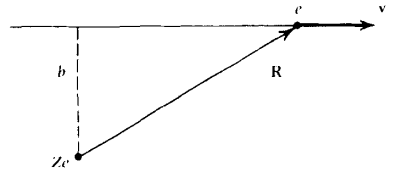
\includegraphics[width=8cm]{brem.png}
\end{center}
\caption{Un electrón pasando por un campo de Coulomb generado por un ión.}\label{bremm}
\end{figure}

La emisividad se verá afectada de acuerdo con la velocidad a la que se encuentre el electrón a la hora de la interacción, para corregir los efectos relativistas se usa el factor de Gaunt. Este factor es una cierta función de la energía de un electrón y de su frecuencia de emisión. En la figura \ref{gaunt} se muestra los diversos regímenes que puede tomar el factor de Gaunt en función de la energía de los electrones.

\begin{figure}[!htbp]
\begin{center}
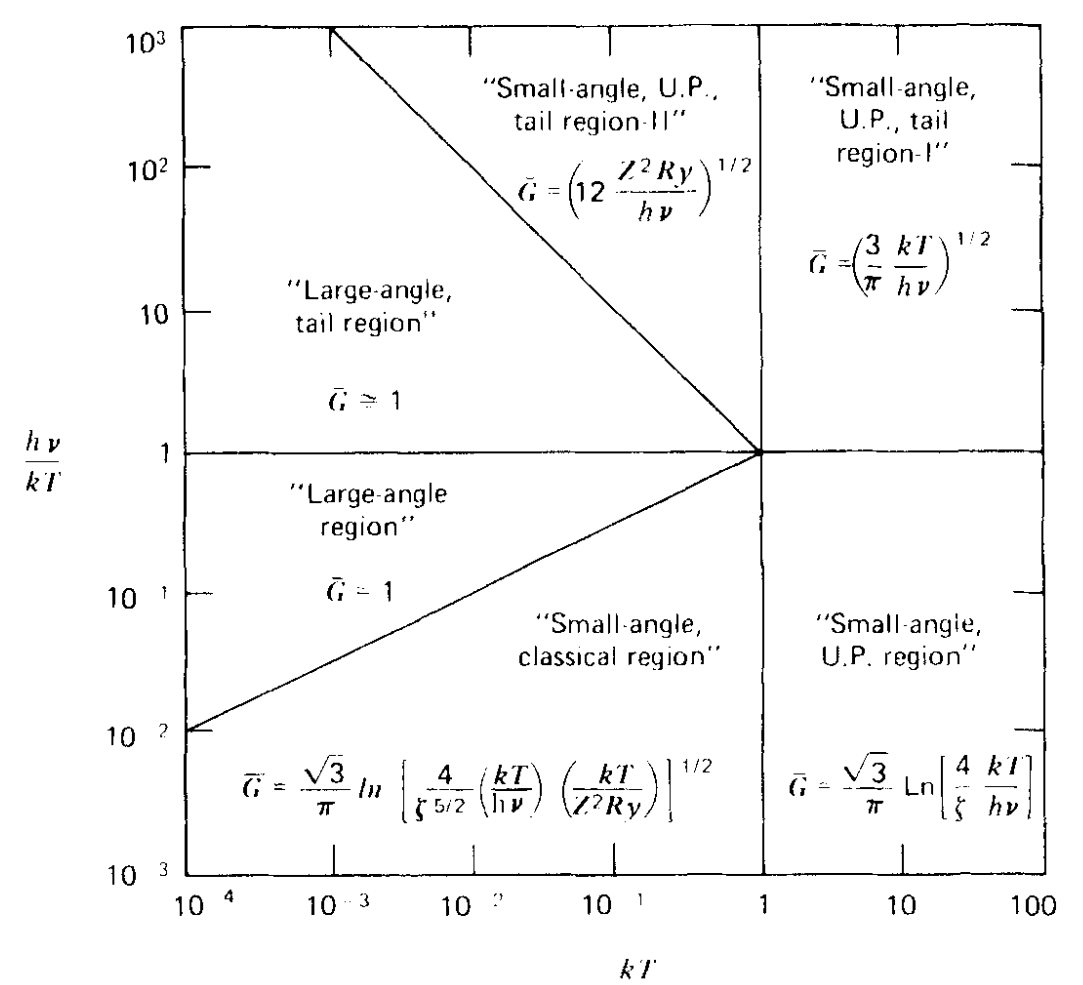
\includegraphics[width=8cm]{gaunt.png}
\end{center}
\caption{Aproximación analítica a el factor de gaunt.}\label{gaunt}
\end{figure}

Usando una aproximación Maxwelliana de velocidades tenemos que la emisión se puede aproximar a

\begin{equation}\label{eq14}
    \kappa_\nu \approx 9.78 \times 10^{-3} \frac{n_e}{\nu^2 T^{\frac{3}{2}}} \Sigma_i Z_i^2 n_i \times A
\end{equation}

donde 
\begin{equation*}
A = \left\{
\begin{array}{ll}
18.2 + ln(T^{\frac{3}{2}}) - ln(\nu) & \mbox{ si } T < 2\times 10^5 K\\
24.5 + ln(T) - ln(\nu) & \mbox{ si } T > 2\times 10^5 K
\end{array}
\right.
\end{equation*}

\newpage
\section{Ecuación de SAHA}
La ecuación de Saha relaciona el estado de ionización de un elemento en función de su temperatura y densidad.

Se puede expresar de la siguiente manera

\begin{equation}
    log\frac{N_{i+1}}{N_i} = -0.1761 - log(P_e) + log\frac{u_{i+1}}{u_i} + 2.5 log(T) - \chi_{i, ion} \frac{5040}{T}
\end{equation}

donde

\begin{eqnarray*}
P_e &=& n_e KT\\
u_i &=& \Sigma_n g_i, n exp \left( -\frac{\chi_{i,n}}{kT} \right)
\end{eqnarray*}

lo que nos da como resultado 
\begin{equation*}
    log\frac{N_{i+1}}{N_i} = 15.6826 - log(n_e) + log\frac{u_{i+1}}{u_i} + 1.5 log(T) - \chi_{i, ion} \frac{5040}{T}
\end{equation*}

si definimos 
    $$log\frac{N_{i+1}}{N_i} = f_{T,i}(n_e) \Rightarrow N_{i+1} = 10^{f_{T,i}(n_e)} N_i$$

Para saber la contribución de los elementos debemos resolver el siguiente sistema

\begin{eqnarray*}
H^0  &=&  (0.9 * N_{tot}) / (1.0 + 10^{f_{T,H^0}(N_e)} )\\
H^+  &=&  0.9 * N_{tot} - H^0\\
He^0 &=&  0.1 * N_{tot} / (1.0 + 10^{f_{T,He^0}(N_e)}(1.0 + 10^{f_{T,He^+}(N_e)}))\\
He^+ &=&  10^{f_{T,He^0}(N_e)} He^0\\
He^{++} &=& 10^{f_{T,He^+}(N_e)} He^+ \\
Ne   &=& H^+ + He^+ + 2*He^{++} 
\end{eqnarray*}

Una vez que se resuelve este sistema podemos conocer la taza de ionización.

\begin{figure}[!htbp]
\begin{center}
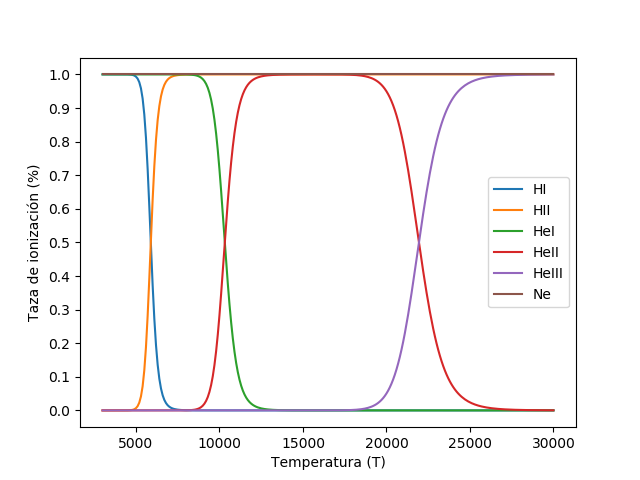
\includegraphics[width=7cm]{saha.png}
\end{center}
\caption{Taza de ionización en función de la temperatura y densidad para diferentes elementos.}\label{saha}
\end{figure}

\newpage
\section{Ley de Planck}

Una aproximación que es fundamental para este código, es asumir que todo está en equilibrio termodinámico, de otra manera la función de emisión Bremmstrahlung estaría descrita de otra manera y la dinámica del sistema en general sería distinta. 

Si suponemos el LTE, podemos usar como función fuente $S_\nu$ a la ley de Planck.
La "Radiación de cuerpo negro"  se refiere a un objeto o sistema que absorbe toda la radiación incidente sobre él, y re-irradia energía que es característica solamente de este sistema radiante, no dependiendo del tipo de radiación que incide sobre ella. La energía radiada puede considerarse que está producido por ondas estacionarias, o modos resonantes de la cavidad que está irradiando.

\begin{figure}[!htbp]
\begin{center}
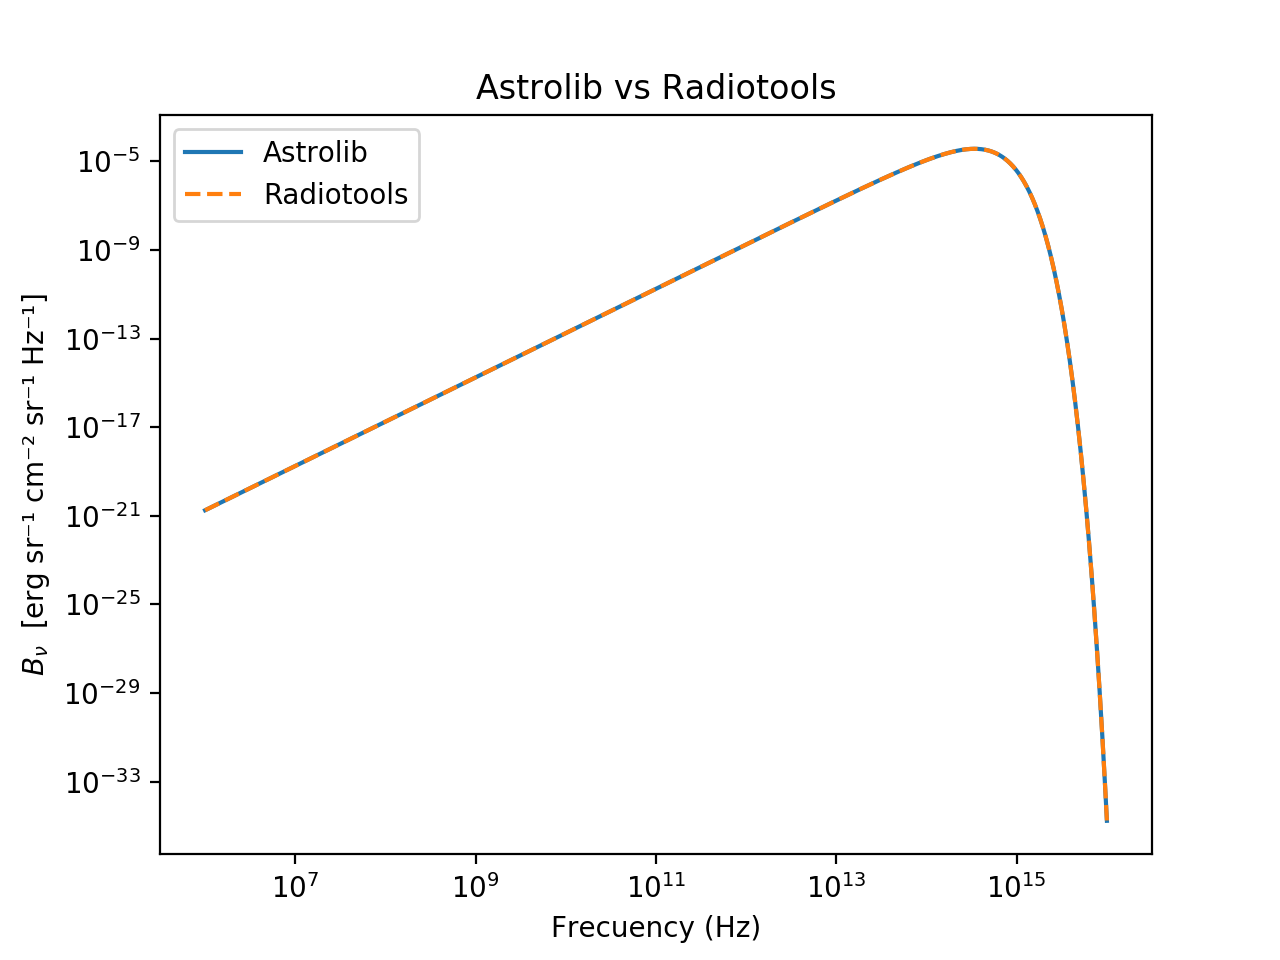
\includegraphics[width=15cm]{asvsrt.png}
\end{center}
\caption{Comparación de Astrolib y RadioTools.}\label{planck}
\end{figure}

\newpage
\section{Código Numérico}

El código numérico se realizó en Julia. El nombre del proyecto es RadioTools.jl y se puede bajar desde (https://github.com/fratava/RadioTools.jl) para instalarlo hay que entrar desde la línea de comandos de Linux o MAC y escribir

\begin{verbatim}
    julia
    
    Pkg.clone("https://github.com/fratava/RadioTools.jl")
    
    using RadioTools
\end{verbatim}

Para generar un espectro sintético se debe dar las siguientes instrucciones

\begin{verbatim}
    I$_\nu$ = intensity(N, $\nu$, T, D, I0)
    
    Tb = tb(I$_\nu$, $\nu$)
\end{verbatim}

donde

\begin{itemize}
    \item N es la densidad electrónica
    \item $\nu$ es la frecuencia que se desea saber la intensidad
    \item T es la temperatura
    \item D es la distancia característica
    \item I0 es la intensidad inicial
\end{itemize}

Pero Radio tools también se puede utilizar para diferentes cosas como
\begin{itemize}
    \item angulares($\lambda$, D; arcs = true) Resolución angular del telescopio para un frecuencia y un diámetro dado en arcosegundos.
    \item rms($\lambda$) El rms mínimo de la antena para un frecuencia dada.
\end{itemize}

\begin{figure}[!htbp]
\begin{center}
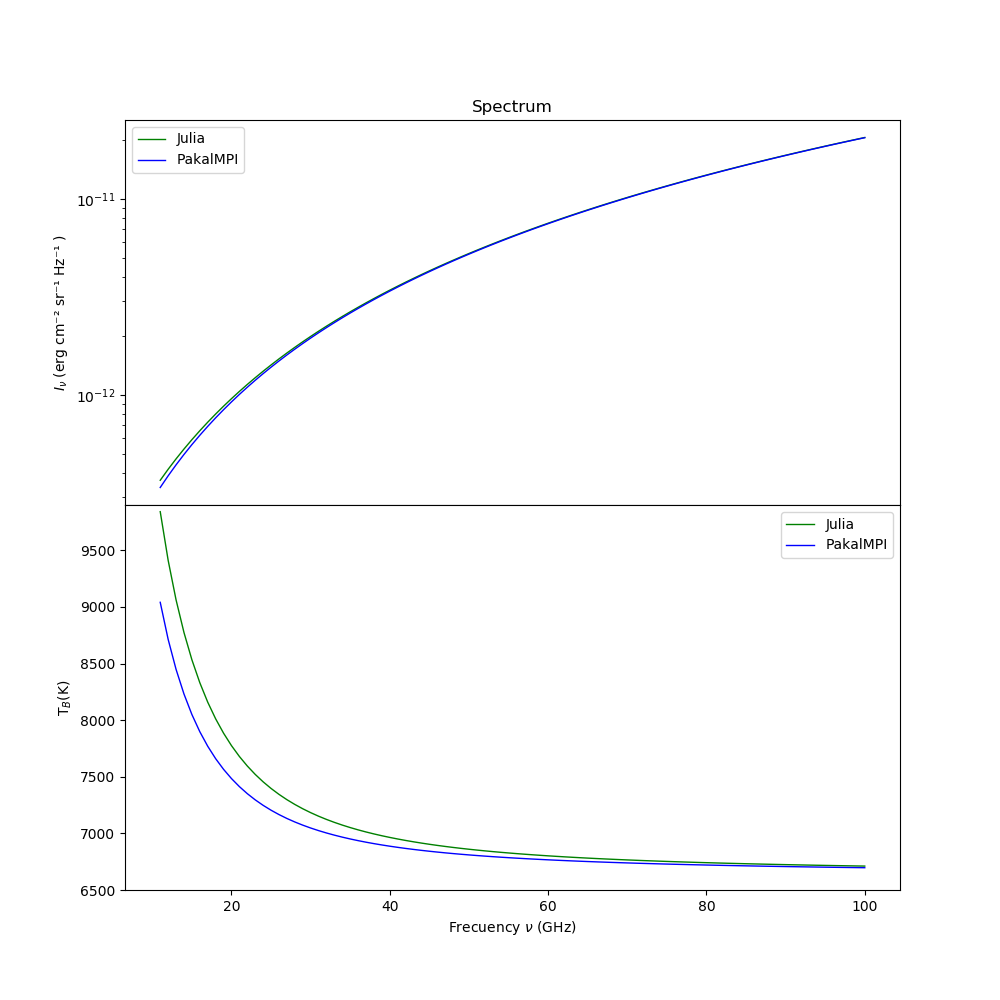
\includegraphics[width=15cm]{rtvspk.png}
\end{center}
\caption{En la parte superior se ve el espectro sintético generado por RadioTools.jl y debajo se comparan las temperaturas de brillo de PakalMPI y RadioTools.jl. Este análisis se hizo para frecuencias que van desde los 11 hasta los 100 GHz}\label{lines}
\end{figure}

\newpage
\section{Caso de prueba}
Para probar la fiabilidad del paquete, es necesario hacer pruebas y compararlas con los resultados que se esperarían. En este caso la primer prueba es sobre la función fuente $S_\nu$. En la figura \ref{planck} se puede ver que la curva es igual a la curva de Plack para todas las frecuencias. 

Una prueba importante es pasar la intensidad específica a temperatura de brillo o $T_b$. Esta prueba es un estándar en todos los radios telescopios del mundo, ya que debido a sus características técnicas no todos reciben la misma cantidad de radiación, sin embargo, eso no significa que no están viendo el mismo fenómeno y para saber si lo que observan es congruente con los reportado por otros o la teoría. 
La temperatura de brillo nos dice a que temperatura de cuerpo negro corresponde ese flujo en la frecuencia a la que se observa. Se utiliza la siguiente ecuación

$$ Tb = \frac{I_\nu c^2}{2 k_b \nu^2} $$

En la figura \ref{fig:acena} se muestra un comparativo entre el código Pakal-MPI que es un código NLTE para atmósferas estelares observadas a longitudes de onda que van desde el infrarrojo hasta el sub-milimétrico. Se puede observar que la emisión es más alta debido a que no se han tomado en cuenta otros fenómenos físicos como cuando una capa se en cuenta en NLTE. Todas estas pruebas son considerando que la líneas de visión del emisor y el receptor son iguales, es decir, $\theta$ = 0.

Para la siguiente prueba, se compara al código con observaciones reales captadas con el radio-interferómetro ALMA de la estrella de tipo solar $\alpha$ Cen A. Los resultados para altas frecuencias difieren por mucha temperatura, pero recordamos que esta es un primera aproximación para un problema complejo que implica asumir que no estamos en los regímenes clásicos del LTE.

\begin{figure}[!htbp]
\begin{center}
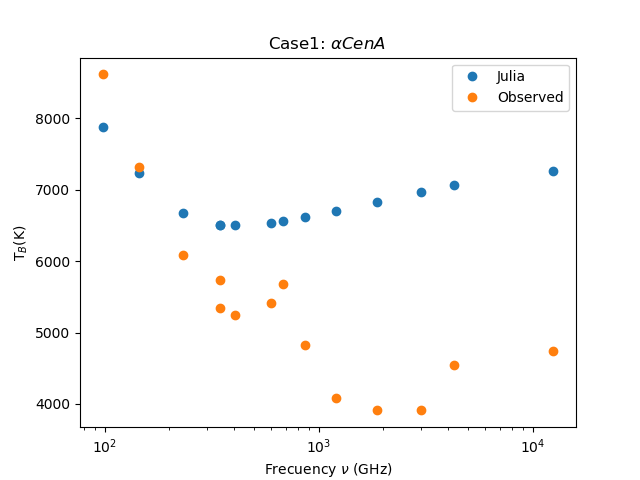
\includegraphics[width=15cm]{acena.png}
\end{center}
\caption{Comparación del espectro sintético contra las observaciones de $\alpha$ Cen A}\label{acena}
\end{figure}

\section{Conclusiones}

En código aquí presentado es una primera aproximación al problema del transporte de energía através de la atmósfera estelar. Para poder obtener los resultados deseados, se tuvo que tener en cuenta 

\begin{itemize}
    \item La taza de ionización de los elementos, la cual es dada por la ecuación de Saha
    \item La función opacidad de Bremsstrahlung para la interacciones entre $e^-$ y $e^+$
    \item La profuncidad óptica en función de la opacidad
    \item La ley de Planck, suponinedo el equilibrio termodinámico y que está radiando como un cuerpo negro
\end{itemize}

Es importante decir que la profundidad óptica en el contexto astrofísico se refiere a que tan opaco es el medio, es decir, a cuanta radiación pasa por el medio.

Lo anterior es parte de los elementos presentes en la ecuación de transferencia radiativa.

En el caso de pruebas pudimos ver que a bajas frecuencias (80-300 GHz) el comportamiento es muy parecido a los datos que se observan, por lo que concluimos que este ejercicio es una buena primera aproximación.

En las figuras \ref{ne} y \ref{hii} se muestran las densidades de electrones y de hidrógeno ionizado. Estos resultados son coherentes pues desde la fotosfera hasta la cromosfera la densidad baja porque hay un gradiente de temperatura y en la zona de transición hay un aumento brusco seguido de un descenso más controlado. En las figuras \ref{hi} y \ref{hei} vemos que hasta antes de la zona de transición hay un cambio pequeño de densidad, pero, un cambio drástico que termina con baja densidad. Esto nuevamente es lo que esperabamos (figura \ref{saha}) pues al aumentar la temperatura estas especies practicamente desaparecen. Para el caso de las figuras \ref{heii} y \ref{heiii} en la fotosfera y en la cromosfera practicamente son cero, es decir, no tienen ninguna contribución. La historia cambia después de la zona de transción, cuando la temperatura es suficiente para ionizan los núcleos de He y con ello aumenta la densidad de estas poblaciones, algo que la ecuación de saha nos había adelantado (figura \ref{saha}). 

Para la profundidad óptica $\tau$, vemos que a 17 Ghz parte de la cromosfera y toda la corona es ópticamente transparente ($\tau <$ 1) (figura \ref{tau}). En el caso de la intensidad podemos observar que la contribución es proporcional a la temperatura a la que se encuentra, un resultado coherente con la teoría.

En conclusión, observamos que los resultados de las especies son comportamientos esperados y esto nos indica que el código está funcionando de una buena forma.

\begin{figure}[!htbp]
\begin{center}
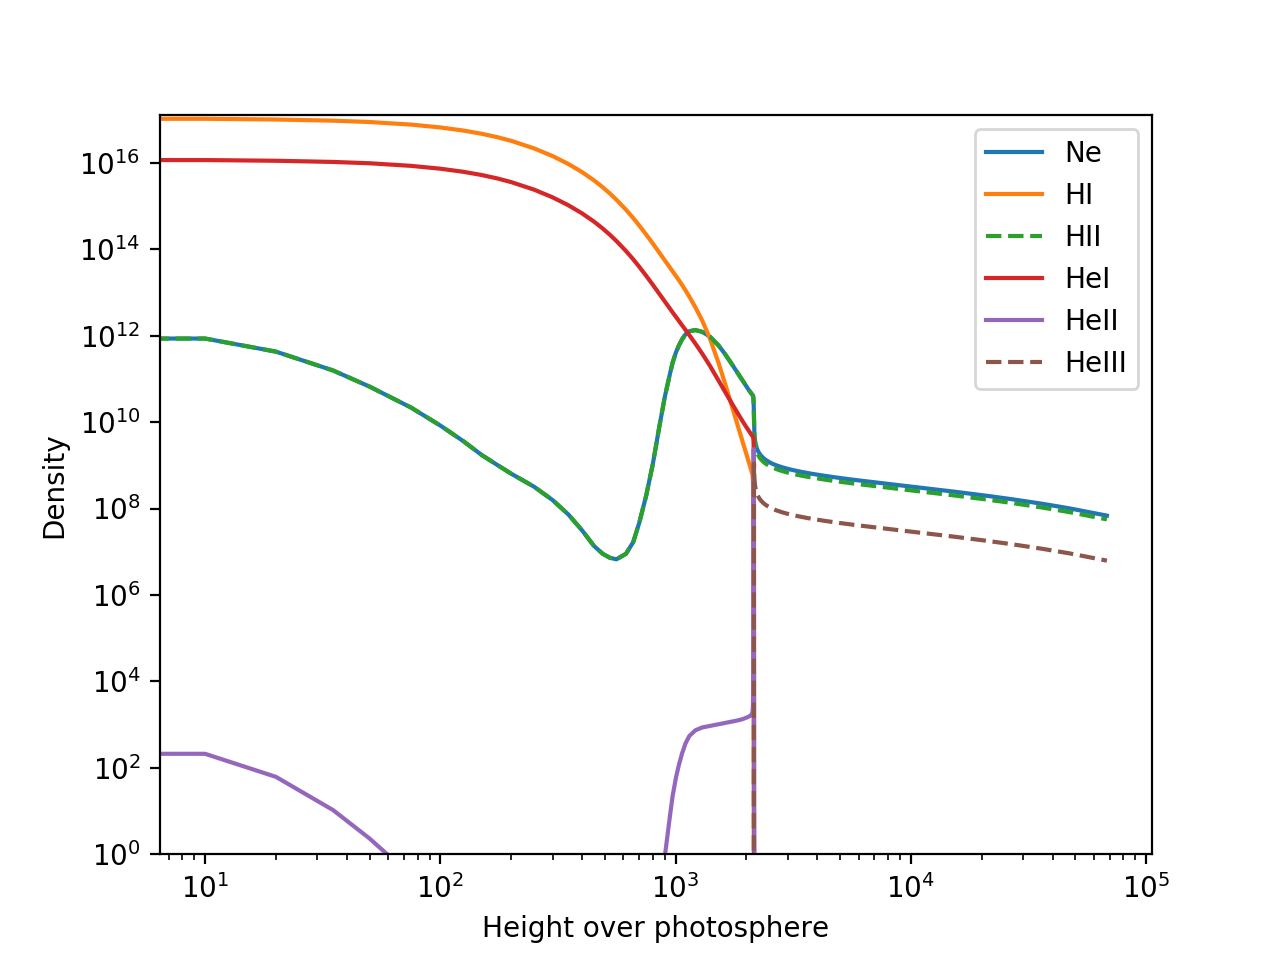
\includegraphics[width=15cm]{esp.png}
\end{center}
\caption{Comparación de especies}\label{ne}
\end{figure}

%\begin{figure}[!htbp]
%\begin{center}
%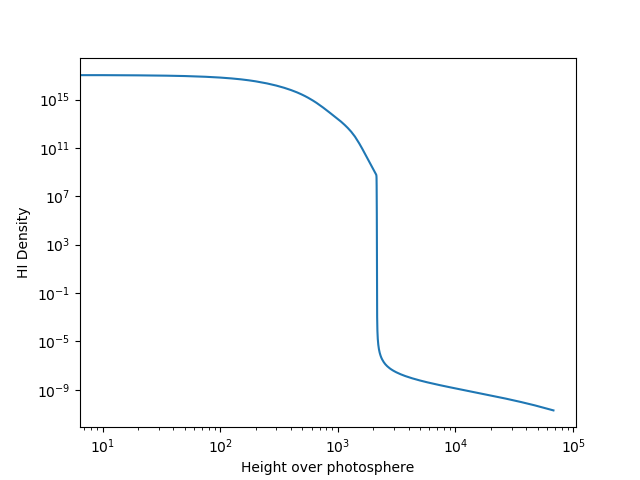
\includegraphics[width=15cm]{HI.png}
%\end{center}
%\caption{Comparación del espectro sintético contra las observaciones de $\alpha$ Cen A}\label{hi}
%\end{figure}


%\begin{figure}[!htbp]
%\begin{center}
%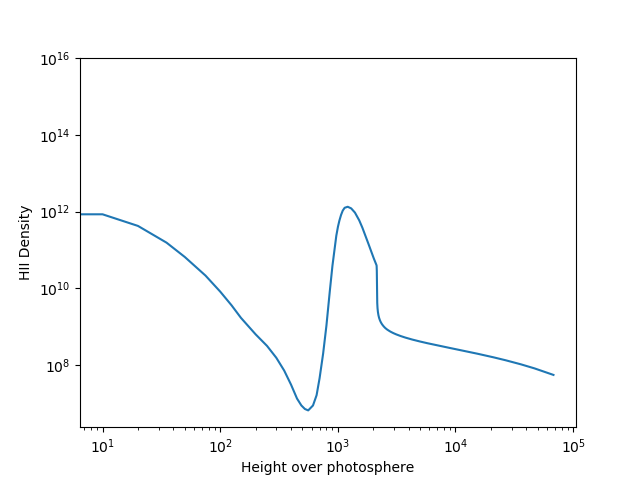
\includegraphics[width=15cm]{HII.png}
%\end{center}
%\caption{Comparación del espectro sintético contra las observaciones de $\alpha$ Cen A}\label{hii}
%\end{figure}


%\begin{figure}[!htbp]
%\begin{center}
%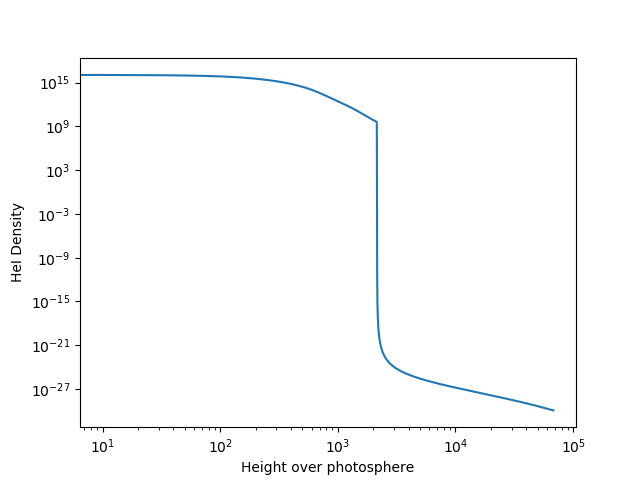
\includegraphics[width=15cm]{HeI.png}
%\end{center}
%\caption{Comparación del espectro sintético contra las observaciones de $\alpha$ Cen A}\label{hei}
%\end{figure}

%\begin{figure}[!htbp]
%\begin{center}
%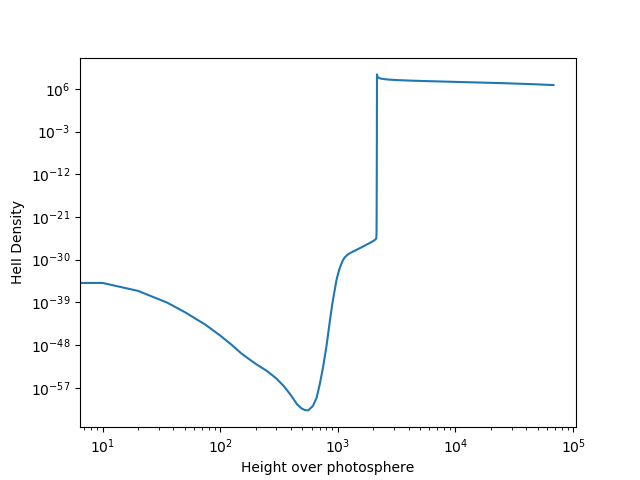
\includegraphics[width=15cm]{HeII.png}
%\end{center}
%\caption{Comparación del espectro sintético contra las observaciones de $\alpha$ Cen A}\label{heii}
%\end{figure}

%\begin{figure}[!htbp]
%\begin{center}
%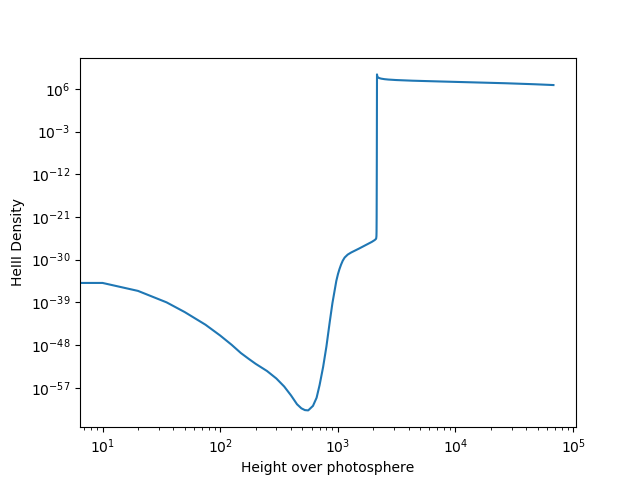
\includegraphics[width=15cm]{HeIII.png}
%\end{center}
%\caption{Comparación del espectro sintético contra las observaciones de $\alpha$ Cen A}\label{heiii}
%\end{figure}

\begin{figure}[!htbp]
\begin{center}
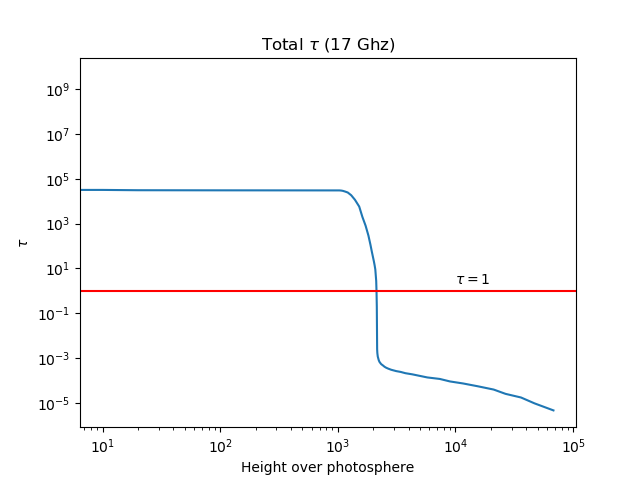
\includegraphics[width=15cm]{tau_total.png}
\end{center}
\caption{Aproximación analítica a el factor de gaunt.}\label{tau}
\end{figure}

\begin{figure}[!htbp]
\begin{center}
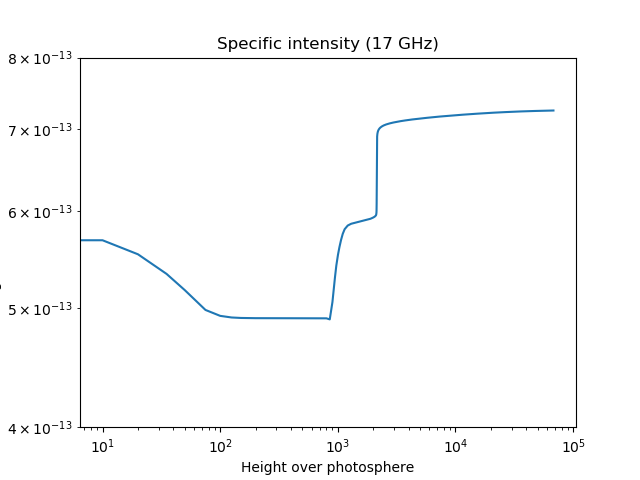
\includegraphics[width=15cm]{ispec.png}
\end{center}
\caption{Aproximación analítica a el factor de gaunt.}\label{ispec}
\end{figure}

%\bibliographystyle{plain}
%\bibliography{bibliography.bib}
\end{document}